\section{Analýza aplikačného rámca pre IPFIX Mediátor} \label{sec:framework}

Analýze aplikačného rámca pre sprostredkovanie správ v IPFIX sa venuje RFC 6183 \citep{rfc6183}. 
V jednotlivých kapitolách si podrobnejšie priblížime referenčný model, vybrané funkčné bloky 
aplikačného rámca a TODO ...

\subsection{Referenčný model sprostredkovania správ v IPFIX}

\begin{figure}[ht!]
\centering
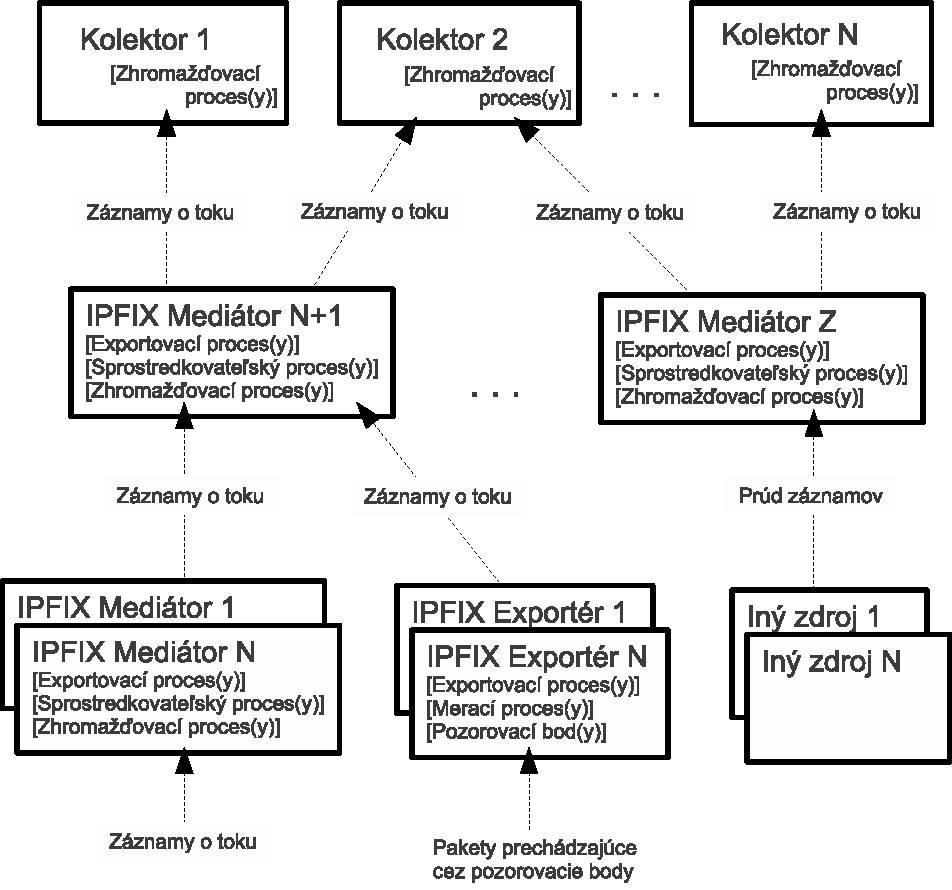
\includegraphics[width=0.9\textwidth]{mediation_reference_model}
\caption{Referenčný model sprostredkovania správ v IPFIX}\label{o:mediation_reference_model}
\end{figure}

Obrázok \ref{o:mediation_reference_model} predstavuje referenčný model sprostredkovania správ v IPFIX 
ako rozšírenie referenčného modelu IPFIX, popísaného v \emph{Architecture for IP Flow Information Export} 
\citep{rfc5470}. Táto schéma zobrazuje možné scenáre, ktoré môžu existovať v meracej architektúre.

Funkčné komponenty v rámci každej entity sú ohraničené zátvorkami []. Mediátor moze prijimat 
zaznamy o toku od inych mediatorov a exporterov a prud zaznamov z inych zdrojov.
Za ine zdroje sa povazuju nastroje inych protokolov, ako napriklad NetFlow exportery \citep{rfc3954}. 
Spracovane data vo forme zaznamov o toku potom exportuje jednemu alebo viacerym kolektorom a mediatorom.

\begin{figure}[ht!]
\centering
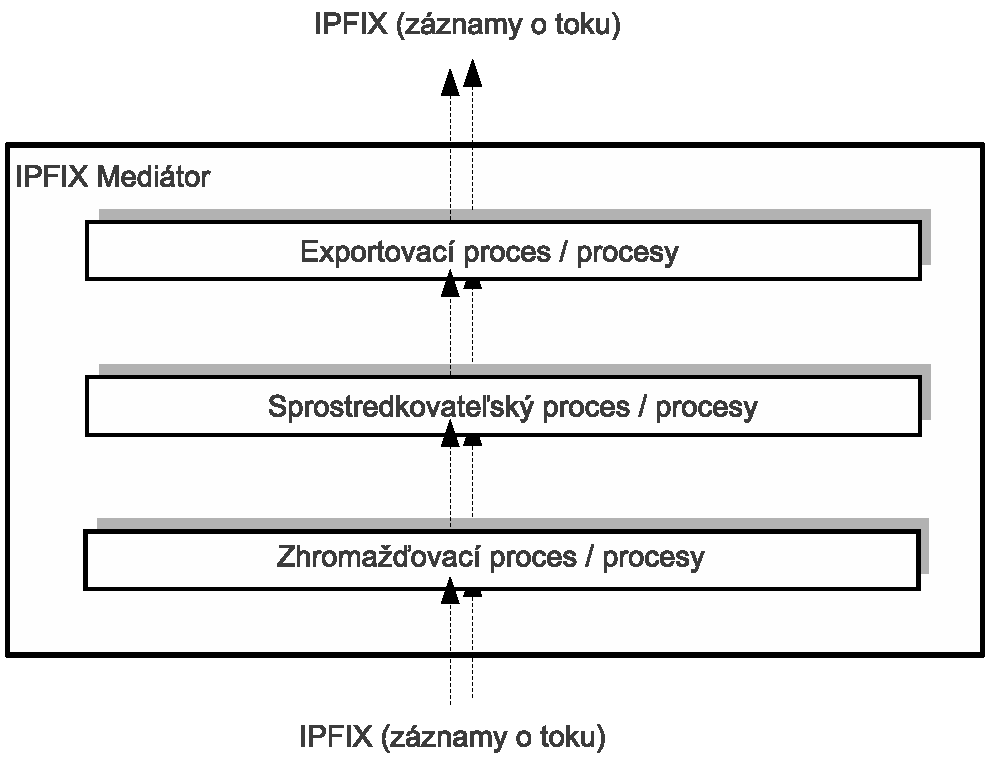
\includegraphics[width=0.7\textwidth]{mediator_component_model}
\caption{Zjednodušený model komponentov IPFIX Mediátora}\label{o:mediator_component_model}
\end{figure}

Zjednoduseny model komponentov IPFIX mediatora je zobrazeny na obrazku \ref{o:mediator_component_model}. 
Mediator obsahuje jeden alebo viac sprostredkovateľských procesov, hierarchicky ulozenych 
medzi jednym alebo viacerymi exportovacimi a zhromazdovacimi procesmi. Tento model sa tyka 
najbeznejsieho pripadu, kedy mediator prijima datove zaznamy od exportera, alebo ineho mediatora.

%% 
%% KED BUDE MALO SEM PRIDAM AJ INE MODELY ... (su este das 3)


\subsection{Komponenty sprostredkovania správ v IPFIX}

V nasleducich castiach si blizsie priblizime jednotlive komponenty IPFIX mediatora, ktore su
znazornene na obrazku \ref{o:mediator_component_model}.

\subsubsection{Zhromazdovaci proces}

Zhromazdovaci proces v IPFIX Mediatore sa nelíši od zhromazdovacieho procesu popisaneho v 
specifikacii IPFIX protokolu \citep{rfc5101}.
Jedinou funkciou naviac je odovzdanie sady dátových záznamov a riadiacich informácii jednemu, alebo 
viacerym komponentom, tj. sprostredkovateľskym procesom, alebo ďalšim aplikáciam. 
To znamena, ze zhromazdovaci proces môže vytvarat kopie sady a prenasat ich bud seriovo, alebo paralelne.  
Medzi riadiace informacie patri hlavicka IPFIX správy, informacie o transportnej relacii, 
spolu s informaciami o meracom a exportovacom procese v exporteri, napr. vzorkovacie parametre.

\subsubsection{Exportovaci proces} \label{sec:exporting_process}

Exportovaci proces IPFIX Mediatora sa vo svojej podstate tiez nelisi od toho, ktory je popisany v specifikacii
protokolu \citep{rfc5101}.
Pridavne funkcie mozu byt nasledujuce:
\begin{itemize}
 \item Prijimat spustac od sprostredkovatelskych procesov, ktory odosle správu kolektoru na odstranenie 
 neplatnej sablony \emph{(Template Withdrawal Message)}.
 \item Z dovodu uvedeneho v kapitole \ref{sec:loss_info} na strane \pageref{sec:loss_info}, je potrebne 
 preposielat informacie o pôvodcovi dat (exporterovi), napriklad ID pozorovacieho bodu a pozorovacej 
 domeny, IP adresa exportera atd. Tieto dáta zakoduje do pridavnych dátovych zaznamov, bud s vyuzitim informacnych
 elementov skupiny 2 (tabulka \ref{t:ie-group2}), alebo organizaciou specifikovanych elementov.
\end{itemize}

% ---- tabulka ----
\tabcolsep=8pt
\begin{table}[!ht]\caption{Prehľad informačných elementov skupiny 2}\label{t:ie-group2}
\smallskip
\centering
\begin{tabular}{|c|c|}
\hline
\textbf{ID} & \textbf{nazov informacneho elementu} \\ \hline
130 & exporterIPv4Address \\ \hline
131 & exporterIPv6Address \\ \hline
217 & exporterTransportPort \\ \hline
211 & collectorIPv4Address \\ \hline
212 & collectorIPv6Address \\ \hline
213 & exportInterface \\ \hline
214 & exportProtocolVersion \\ \hline
215 & exportTransportProtocol \\ \hline
216 & collectorTransportPort \\ \hline
173 & flowKeyIndicator \\ \hline
\end{tabular}
\end{table}
% -----------

\subsubsection{Sprostredkovatelske procesy} \label{sec:framework_intermediate}

Sprostredkovatelske procesy su klucovymi funkcnymi blokmi sprostredkovania správ v IPFIX. Musia pokryt 
kazdy priklad pouzita spostredkovania správ z kapitoly \ref{sec:mediator_examples} na strane 
\pageref{sec:mediator_examples}. 
Mediator musi byť schopný súčasne podporovat viac ako jeden sprostredkovatelsky proces. Spolupraca viacerych 
procesov je konfigurovana nasledujúcimi spôsobmi.

\begin{itemize}
 \item \textbf{Paralelne spracovanie} - Prúd záznamov je spracovaný viacerymi sprostredkovateľskými procesmi paralelne
tak, aby boli splnene požiadavky koncovych aplikácií. V tomto scenare, každy sprostredkovatelsky proces dostava
kópiu celeho prudu zaznamov ako vstup.
 \item \textbf{Seriove spracovanie} - Aby bolo zabezpecene flexibilne spracovanie prudu zaznamov, sprostredkovatelske
 procesy su zapojene seriovo. V tomto pripade vystupny prud zaznamov jedneho procesu je vstupym prudom nasledujuceho 
 procesu.
\end{itemize}






















